\documentclass[../document.tex]{subfiles}
\begin{document}
\chapter{Methodology}
We develop a framework to learn and predict traversability that learns directly on ground patches for any robot using purely simulated data. The main idea is to run a robot into a simulator on different syntetic terrain and later used its interactions to train an estimator. Simulation data has two main advantages: varirity, cost and speed. With simulations, we can easily increase the number of data samples by just include more maps, while doing the same with a real robot requires to first identify the suitable ground and then travel to it. Clearly, this also decrease the time required to collect the robot's interaction with the ground. The time could be additional decreased by running different simulations in paralla avoiding to physical manufactor or buy additional robots. 
Moreover, we are not limited by physical constrain and therefore the robot can interact with a multitude of different grounds. For instance, to collected real world data the robot must be physically transport to different locations, on the other hand, with simulations we can immediately load a new map.

To create a quality dataset, we must first generate a series of various surfaces and ensure their variarity. Intuitivelly, those maps should be small enough to allow a quick interaction with their features but big enough to include variarity. With modern ground generation techiques it is fairly streightforward to generate a rich array of terrains with different characteristics such us bumps, ramps, slopes in different levels and sizes. 
\begin{figure}[H]
    \centering
    \begin{subfigure}[b]{0.24\textwidth}
        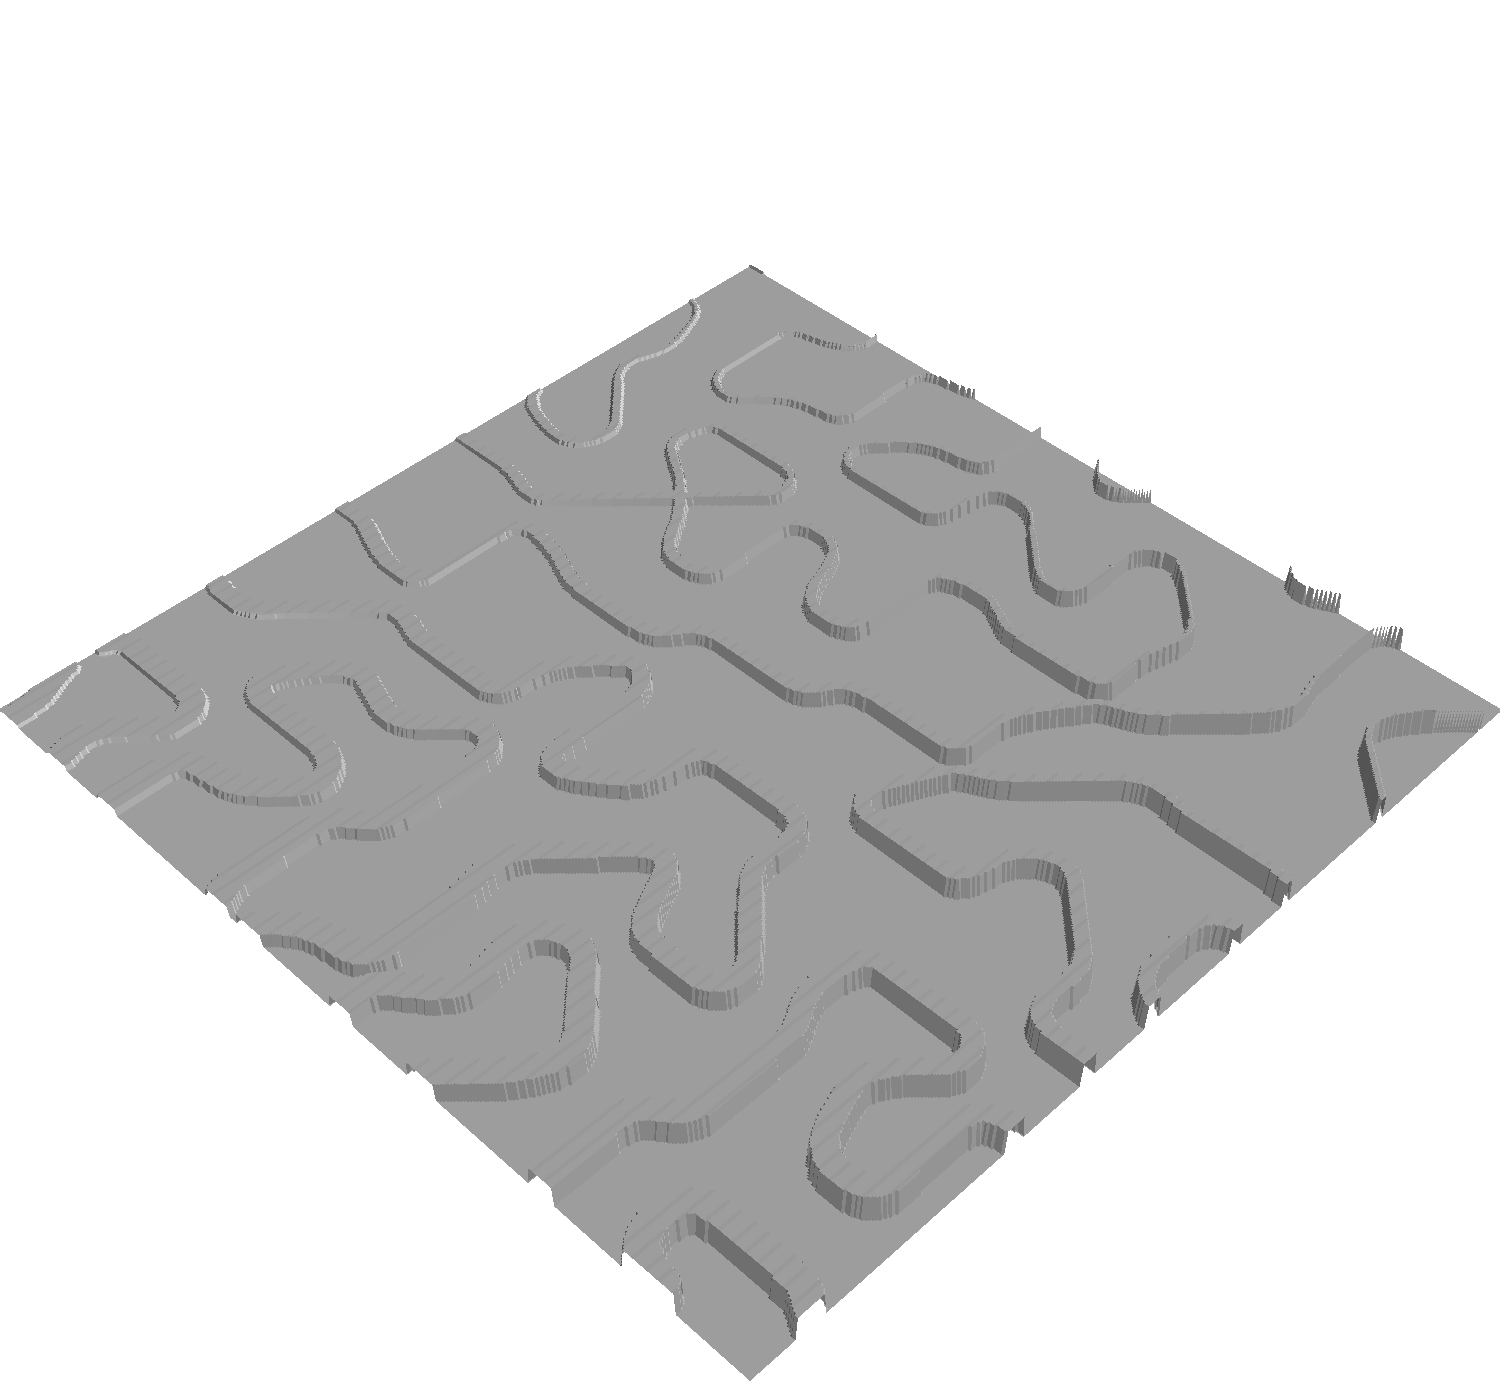
\includegraphics[width=\linewidth]{../img/hm3d/bars1.png}
        \caption{Walls.}
    \end{subfigure}
    \begin{subfigure}[b]{0.24\textwidth}
        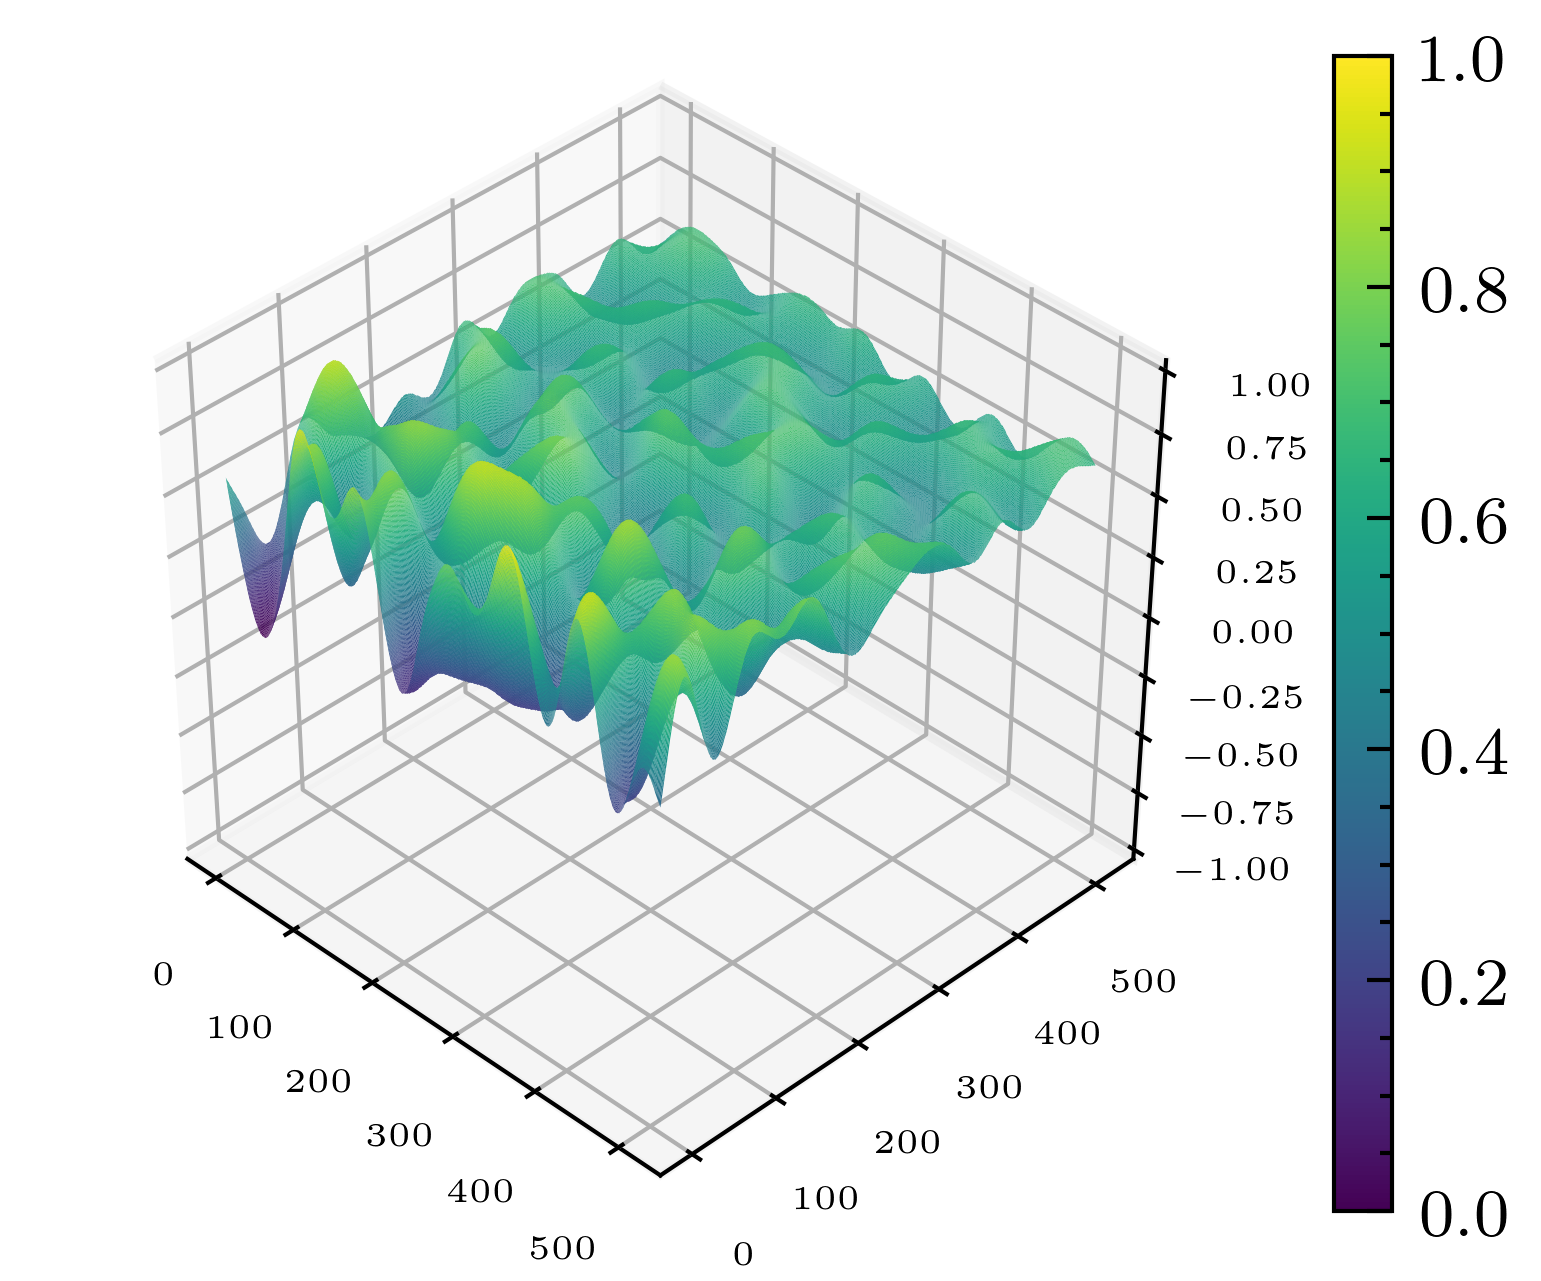
\includegraphics[width=\linewidth]{../img/hm3d/bumps2.png}
        \caption{Bumps.}
 \end{subfigure}  
    \begin{subfigure}[b]{0.24\textwidth}
        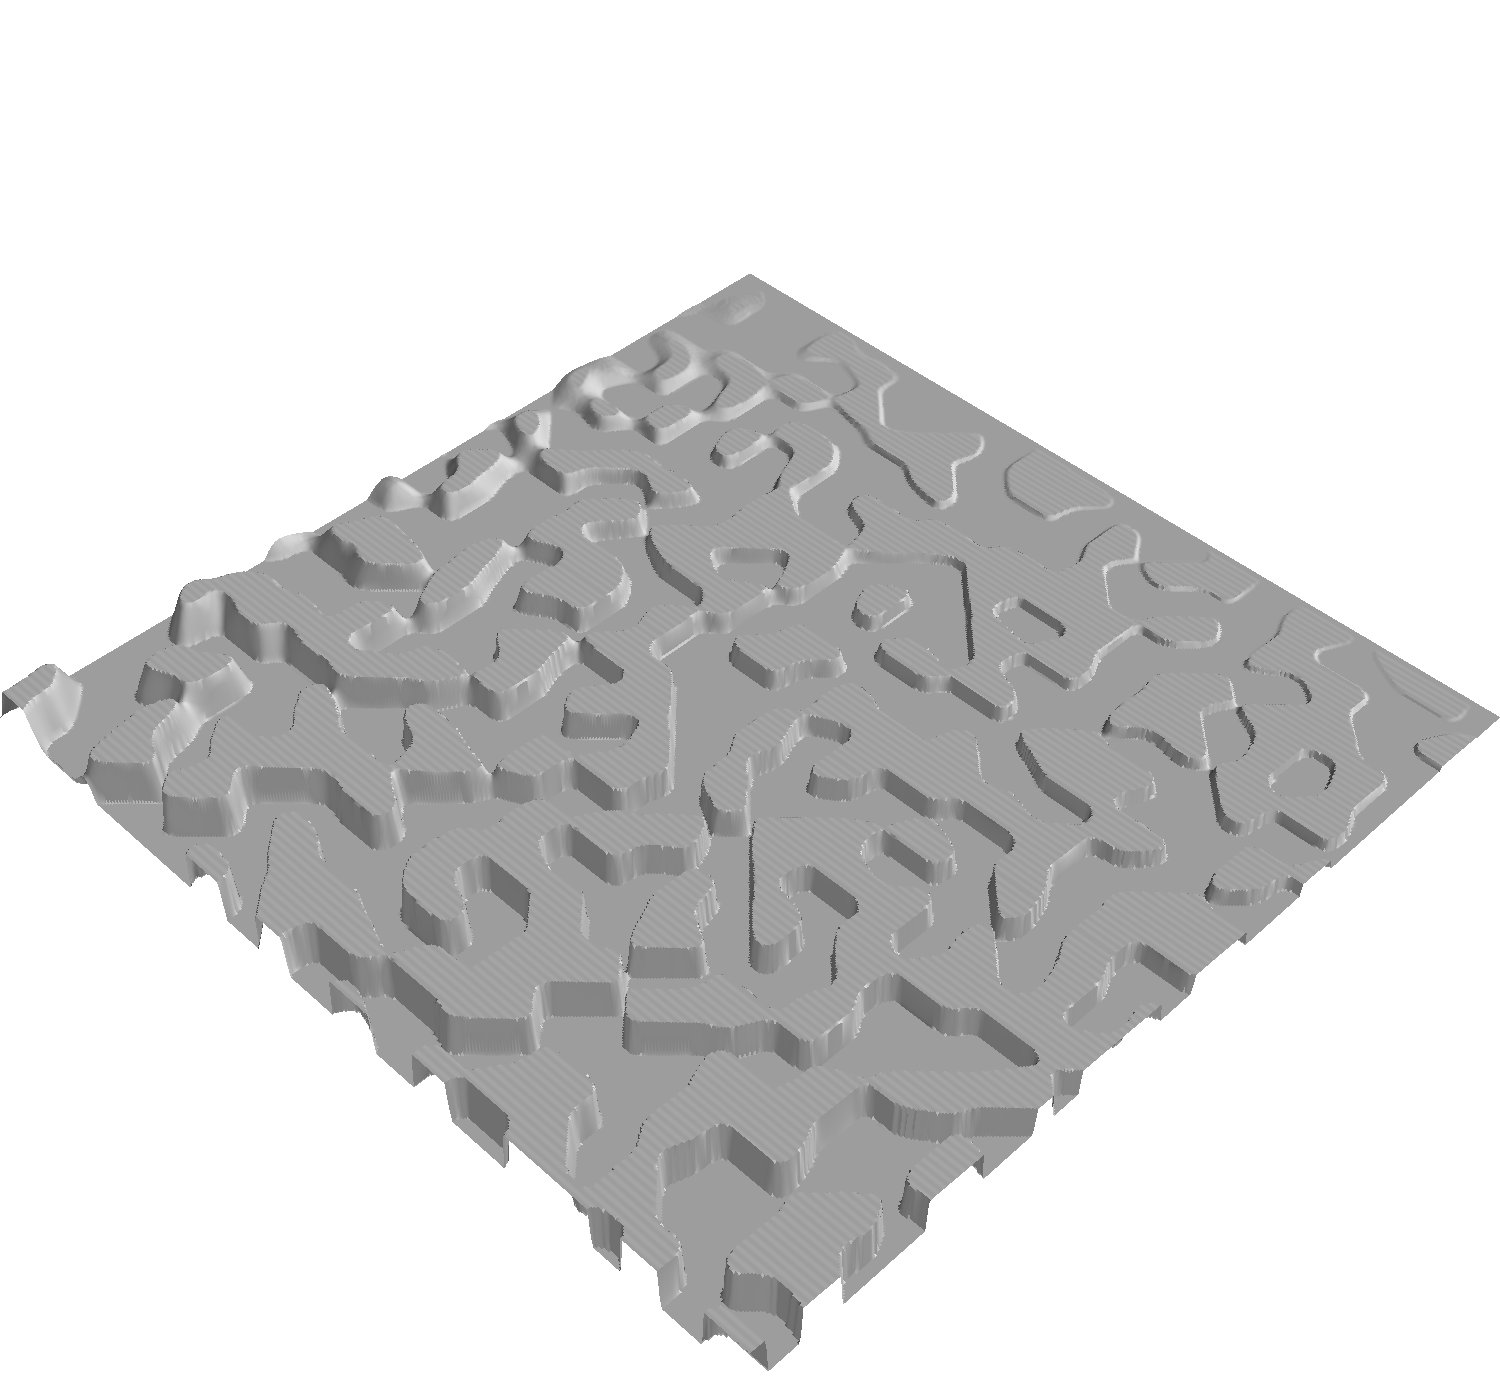
\includegraphics[width=\linewidth]{../img/hm3d/steps1.png}
        \caption{Steps.}
 \end{subfigure}  
    \begin{subfigure}[b]{0.24\textwidth}
        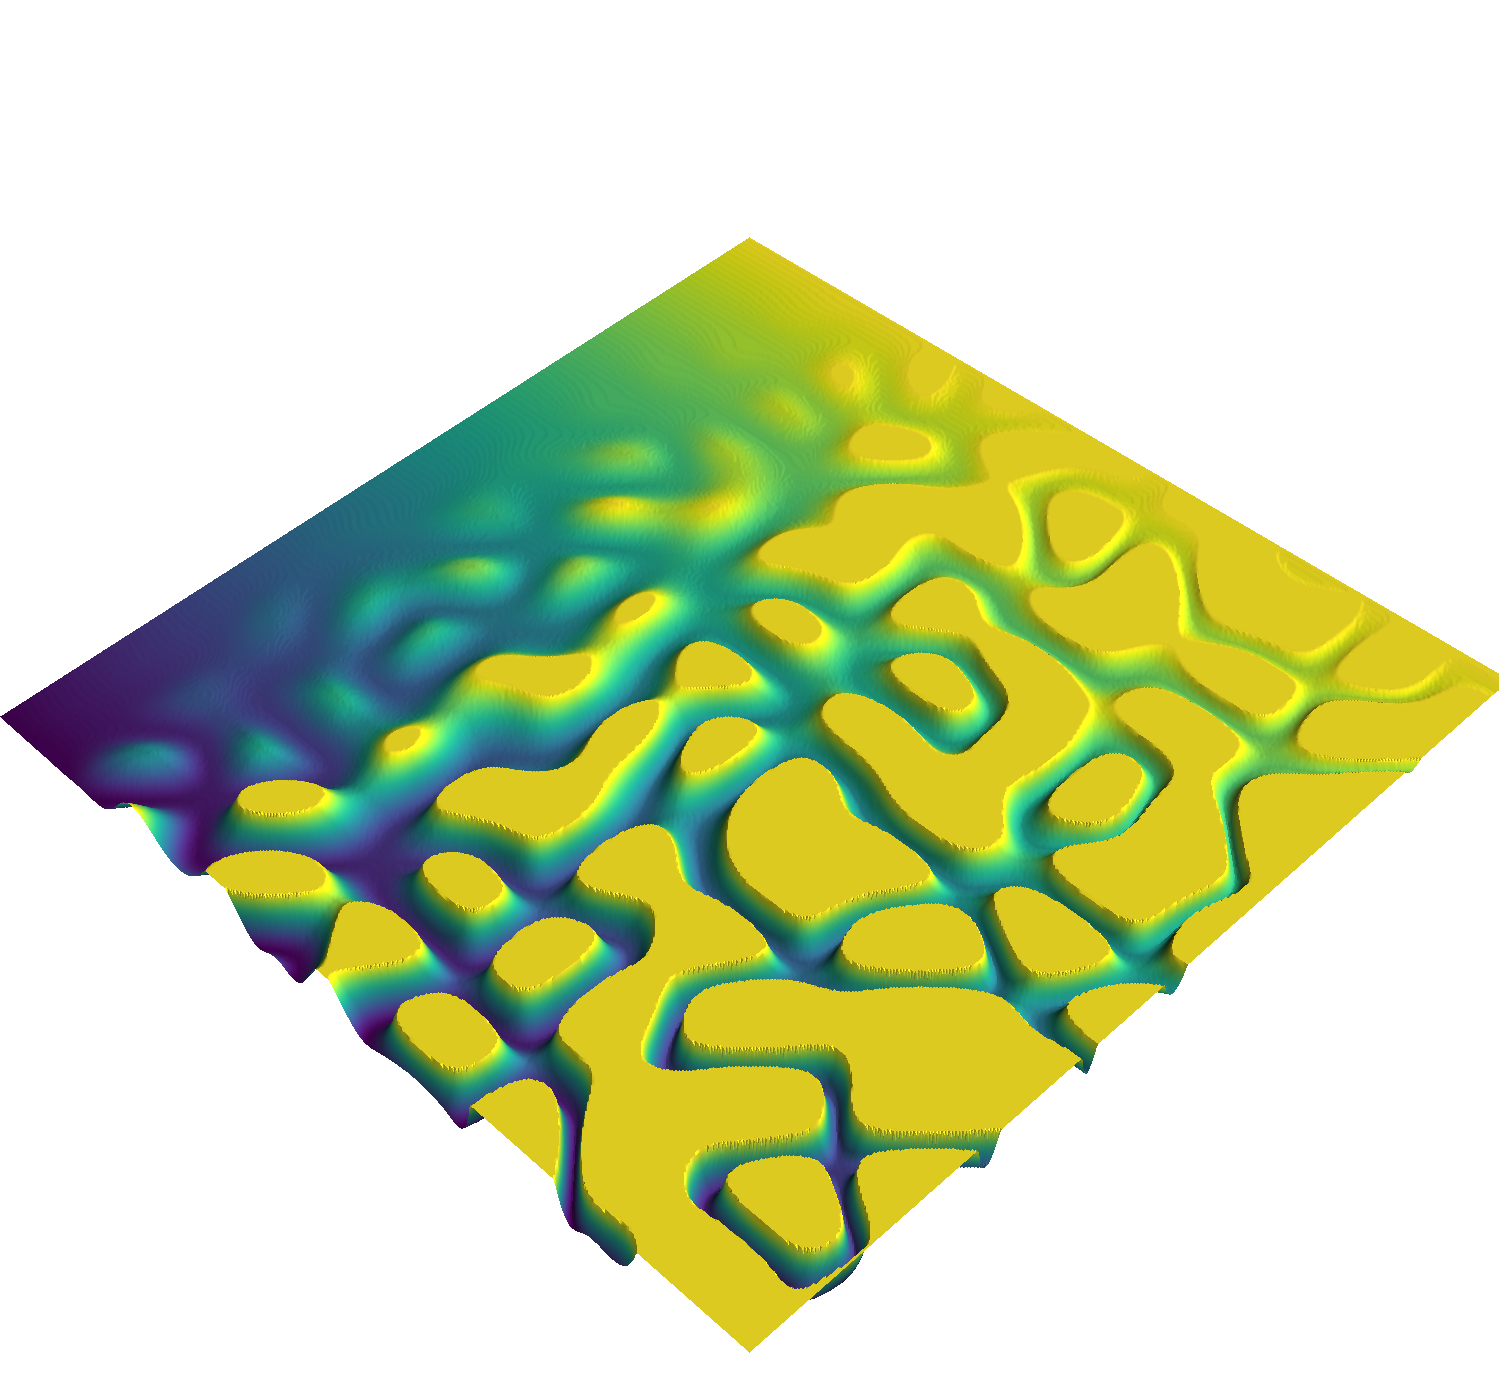
\includegraphics[width=\linewidth]{../img/hm3d/rails3.png}
        \caption{Rails.}
    \end{subfigure}  
\caption{Some artificially generated terrains, $10\times 10$m, with one specific feature each. }   
\end{figure}
This maps can be loaded into a simulator to let the robot interact with them. To ensure a correct exploration of each terrain, it is better to randomly spawn the robot multiple times on the same map and let it walk for a fixed amount of time. The robot position is tracked and stored during simulation in order to extract a small portion of ground, patches, around each of its trajectory's position. Those patches are label using a minimum advancement defined for the robot and then directly feed to a deep neural network. 
\begin{figure}[H]
    \centering
    \begin{subfigure}[b]{1\textwidth}
    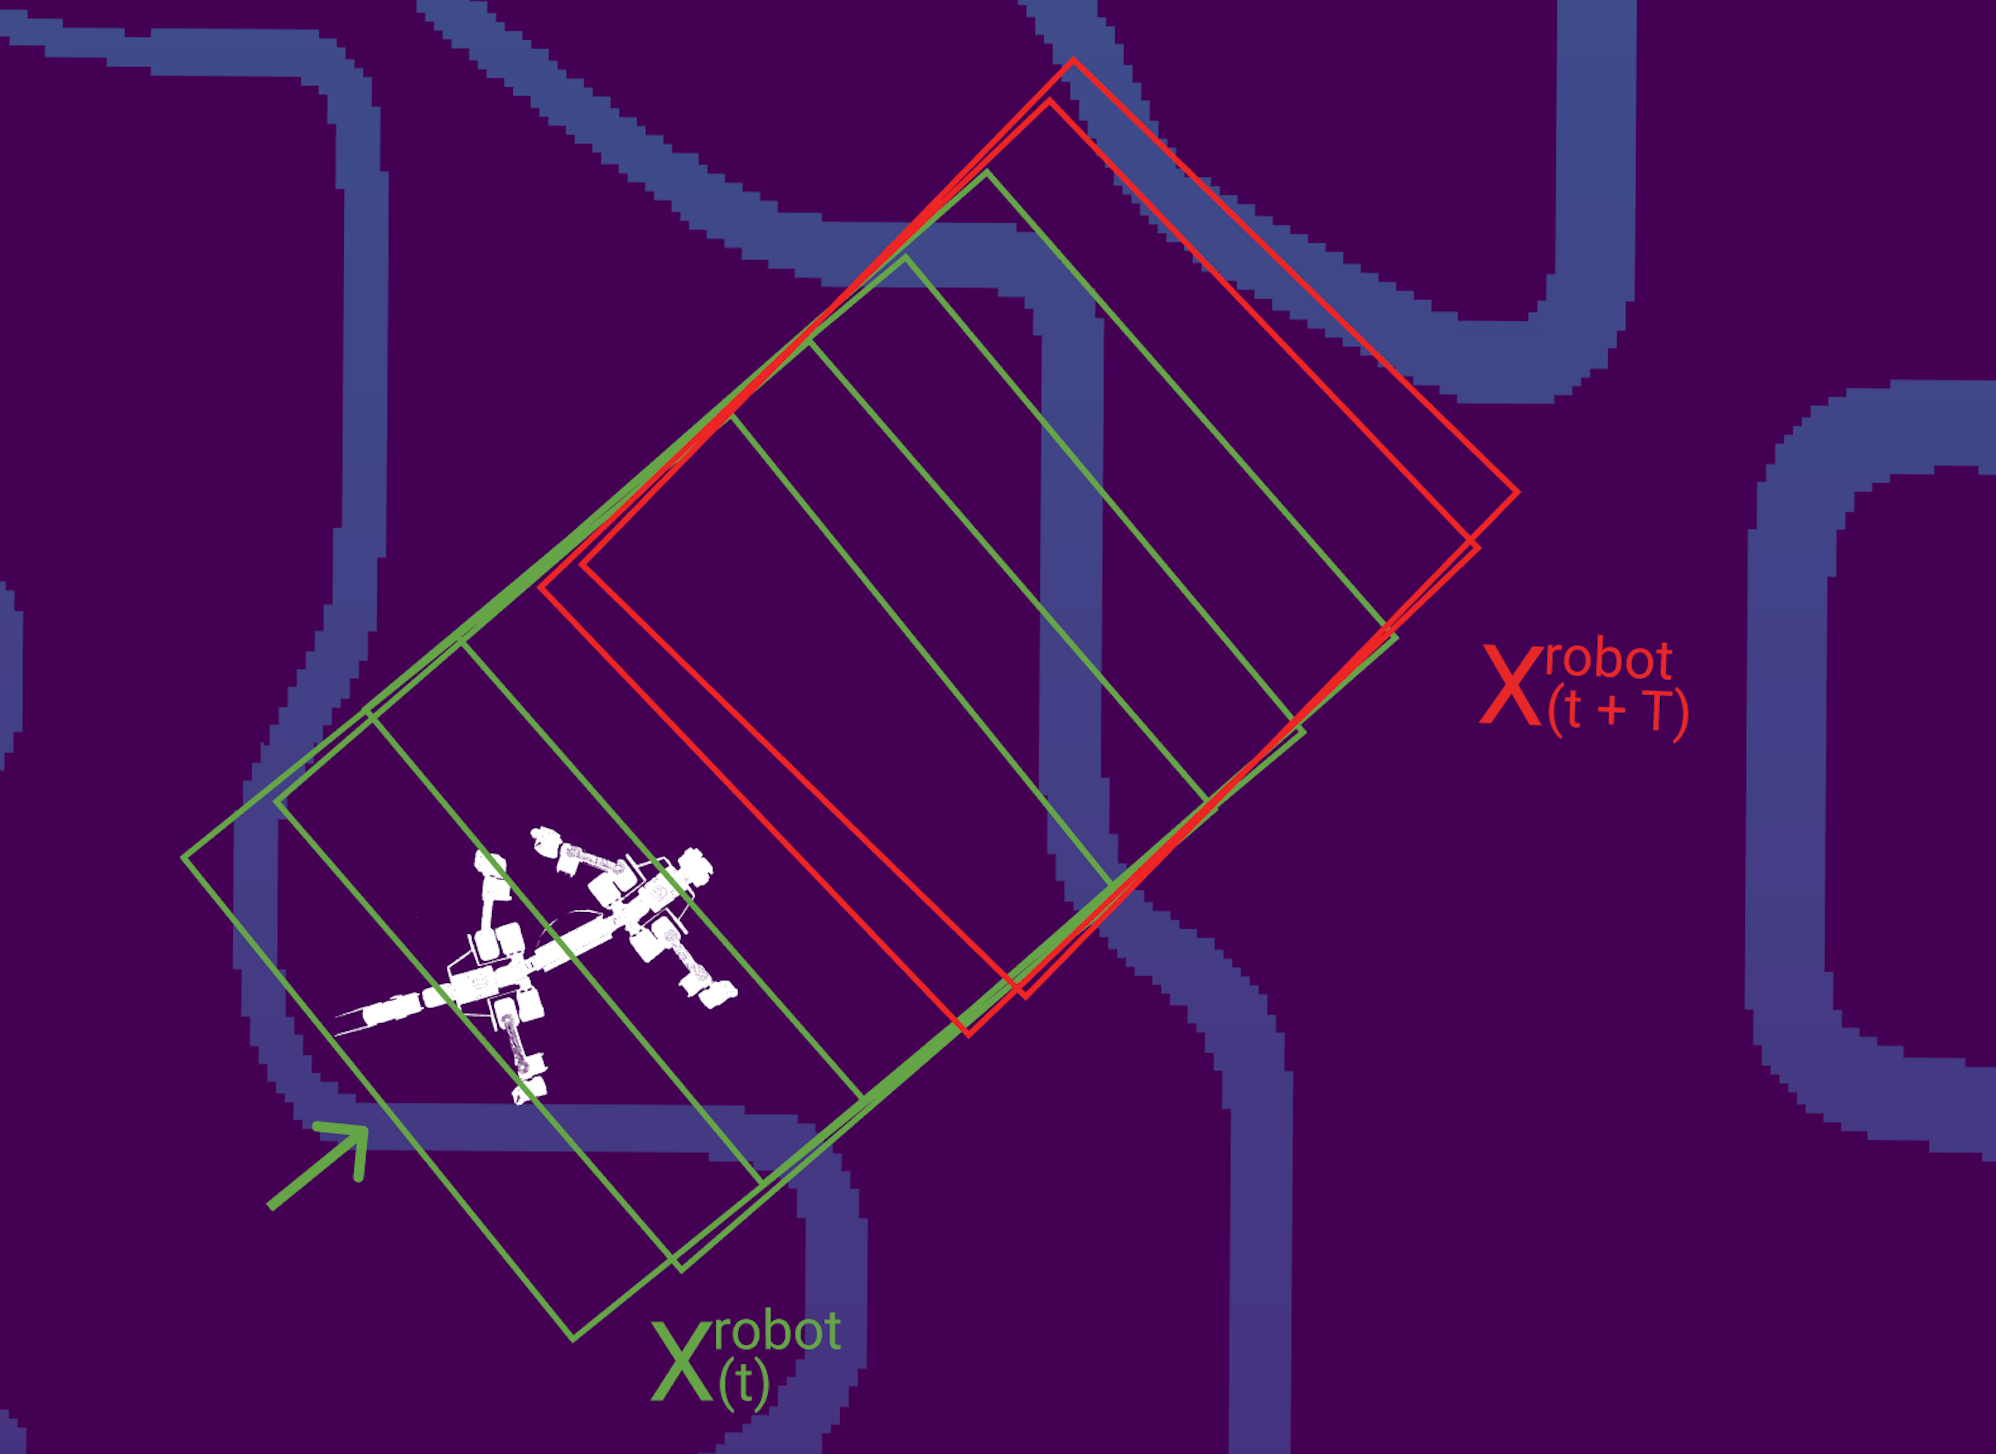
\includegraphics[width=\textwidth]{../img/krock-bars-correct-small.png}
    \caption{Robot's trajectory.}
\end{subfigure}
\begin{subfigure}[b]{1\textwidth}
    \begin{subfigure}[b]{0.19\textwidth}
    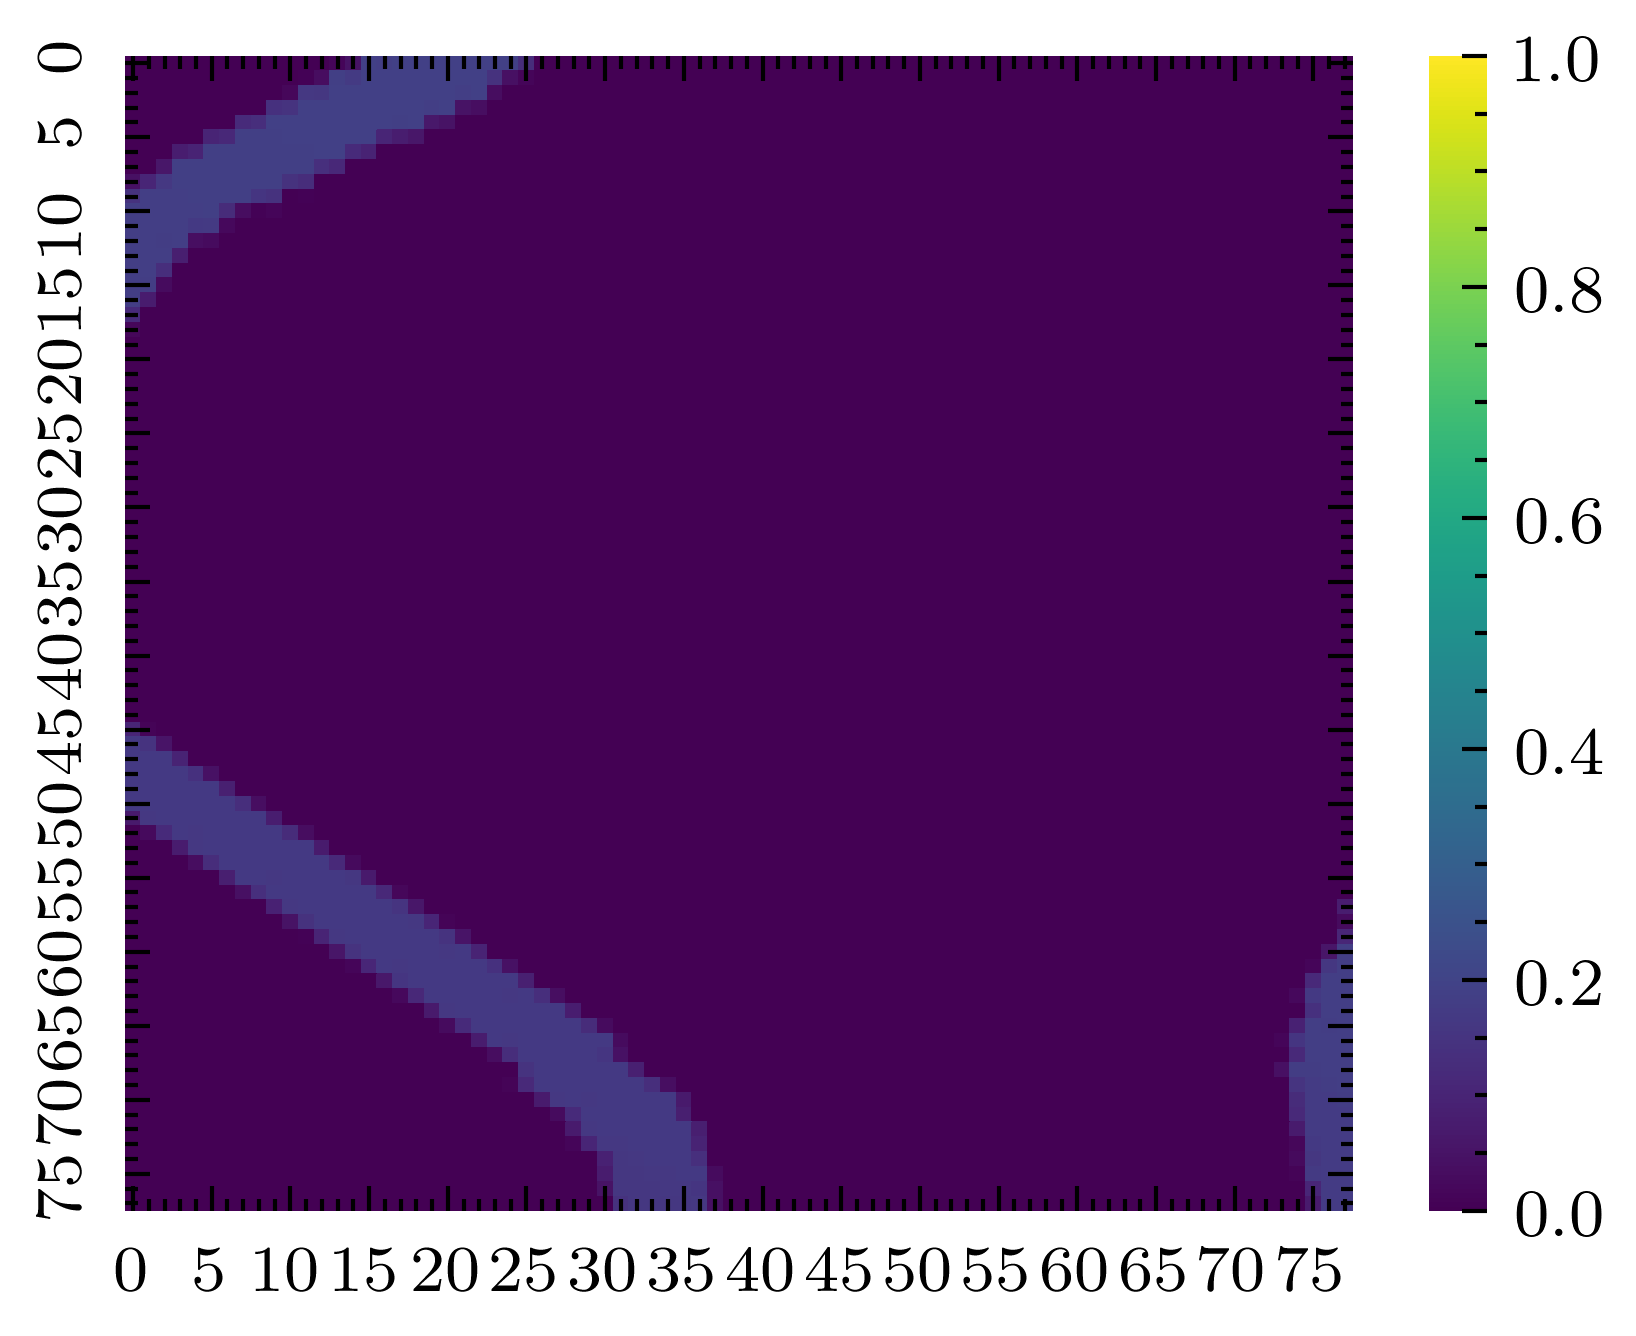
\includegraphics[width=\linewidth]{../img/bars1-example-patches/2d/0.png}
    \end{subfigure}
    \begin{subfigure}[b]{0.19\textwidth}
    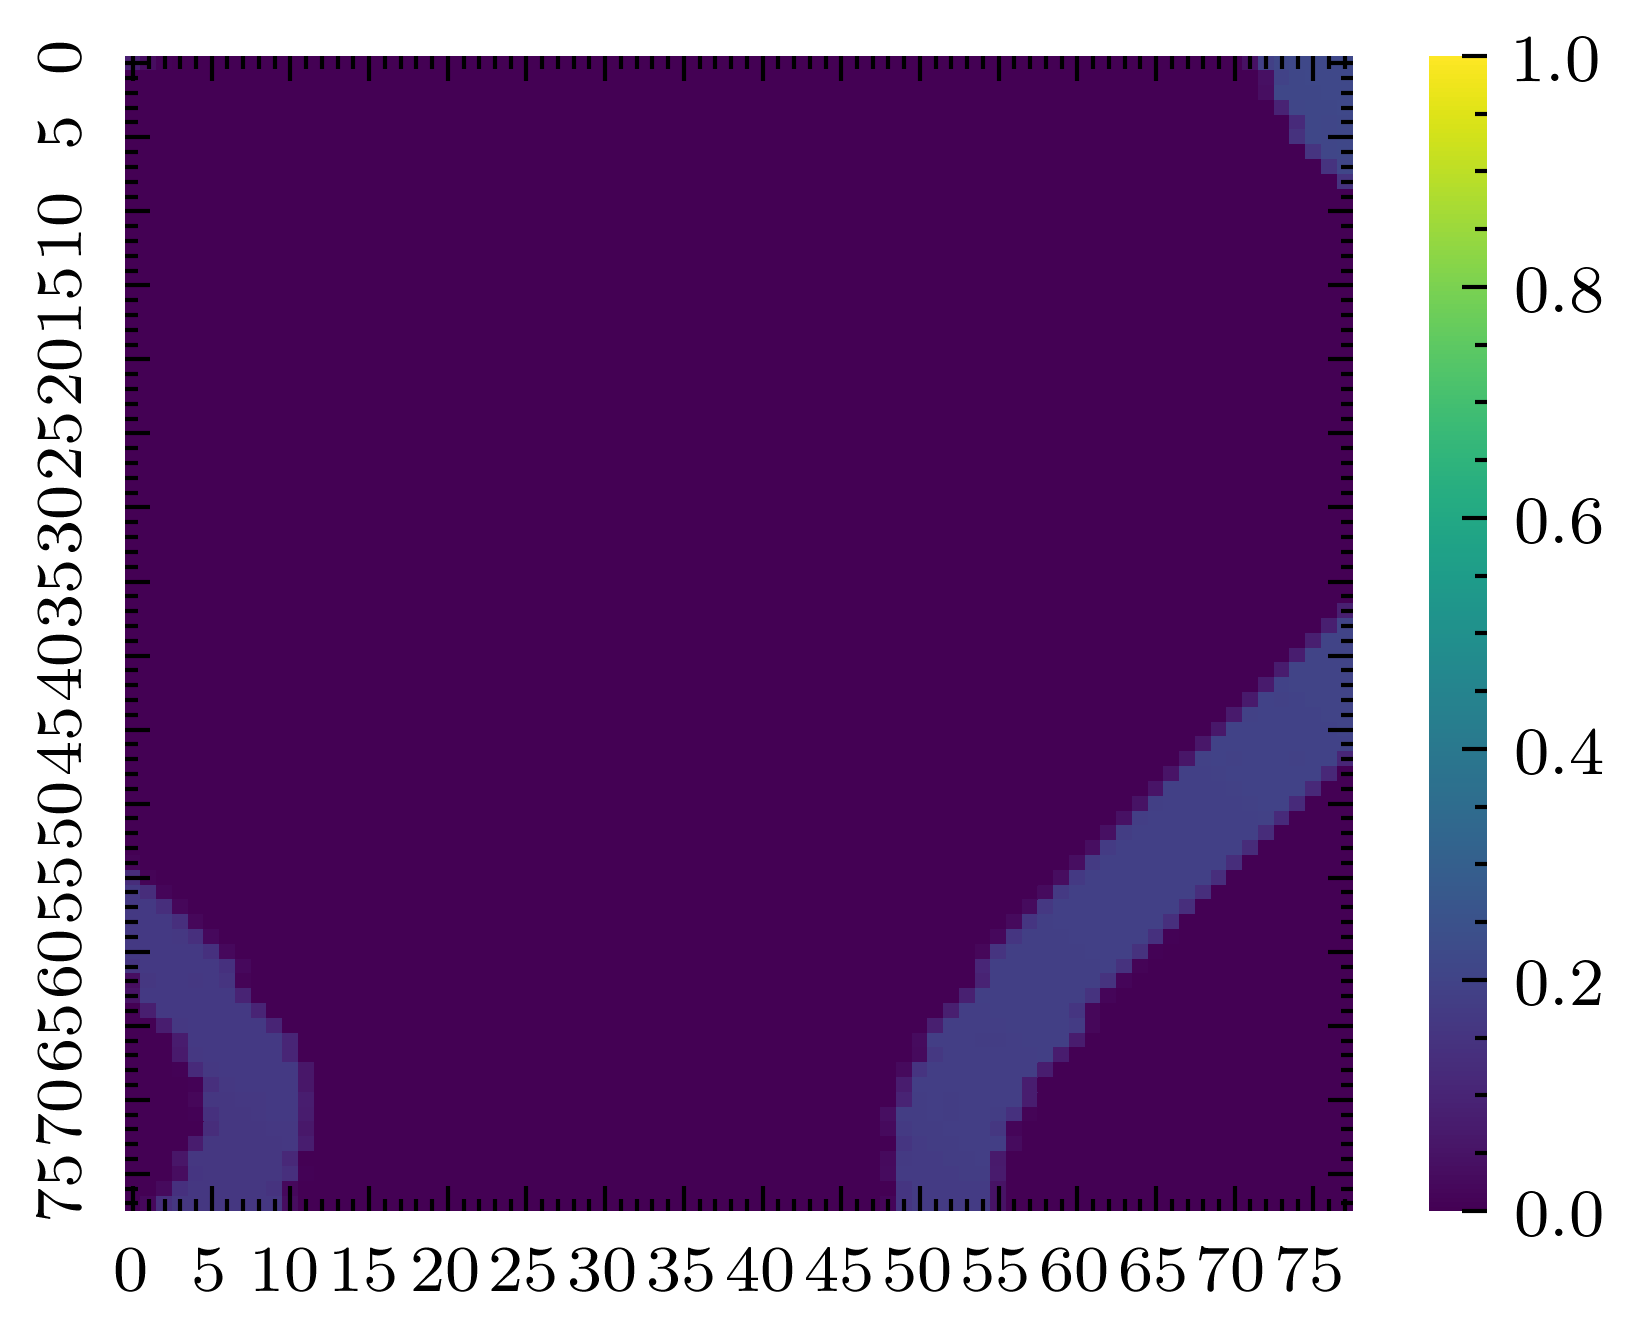
\includegraphics[width=\linewidth]{../img/bars1-example-patches/2d/2.png}    
    \end{subfigure}  
    \begin{subfigure}[b]{0.19\textwidth}
    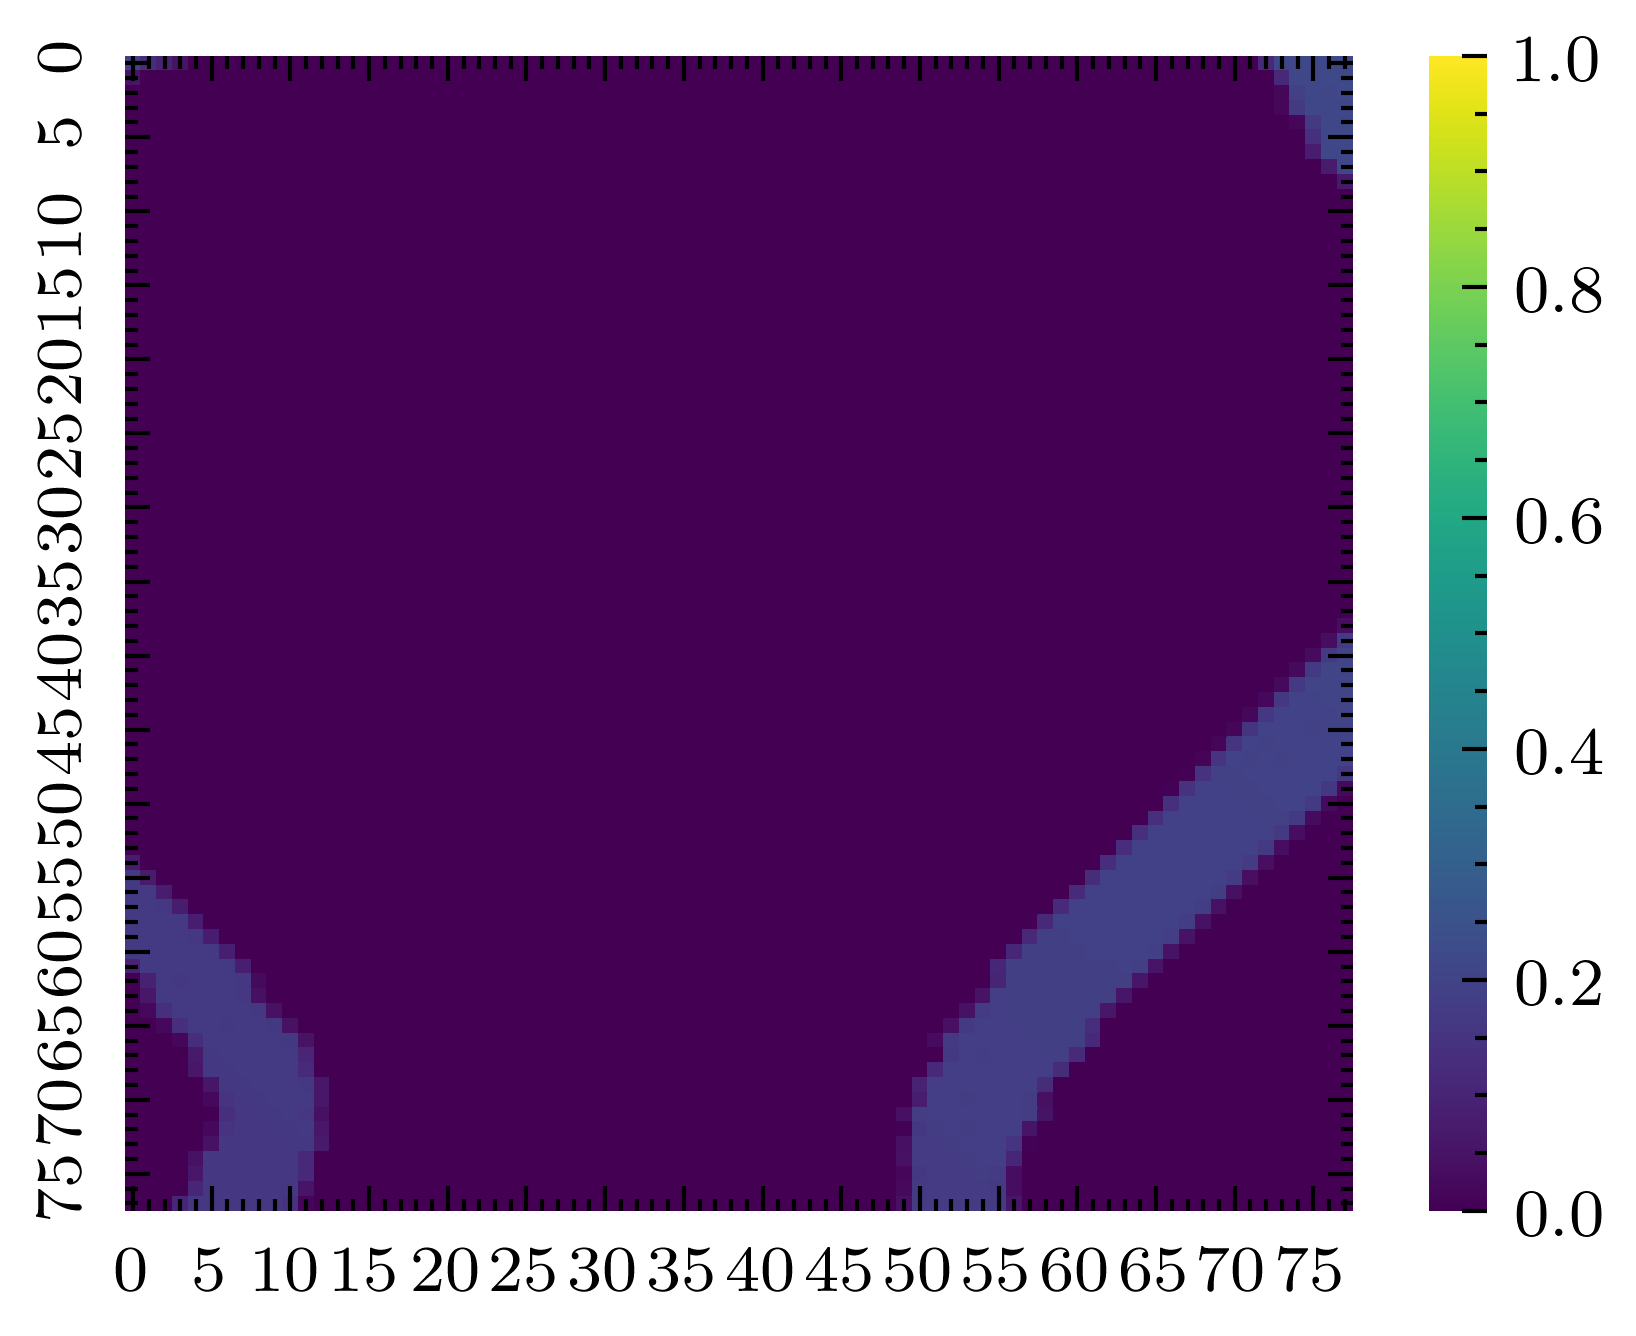
\includegraphics[width=\linewidth]{../img/bars1-example-patches/2d/4.png} 
    \end{subfigure}
    \begin{subfigure}[b]{0.19\textwidth}
    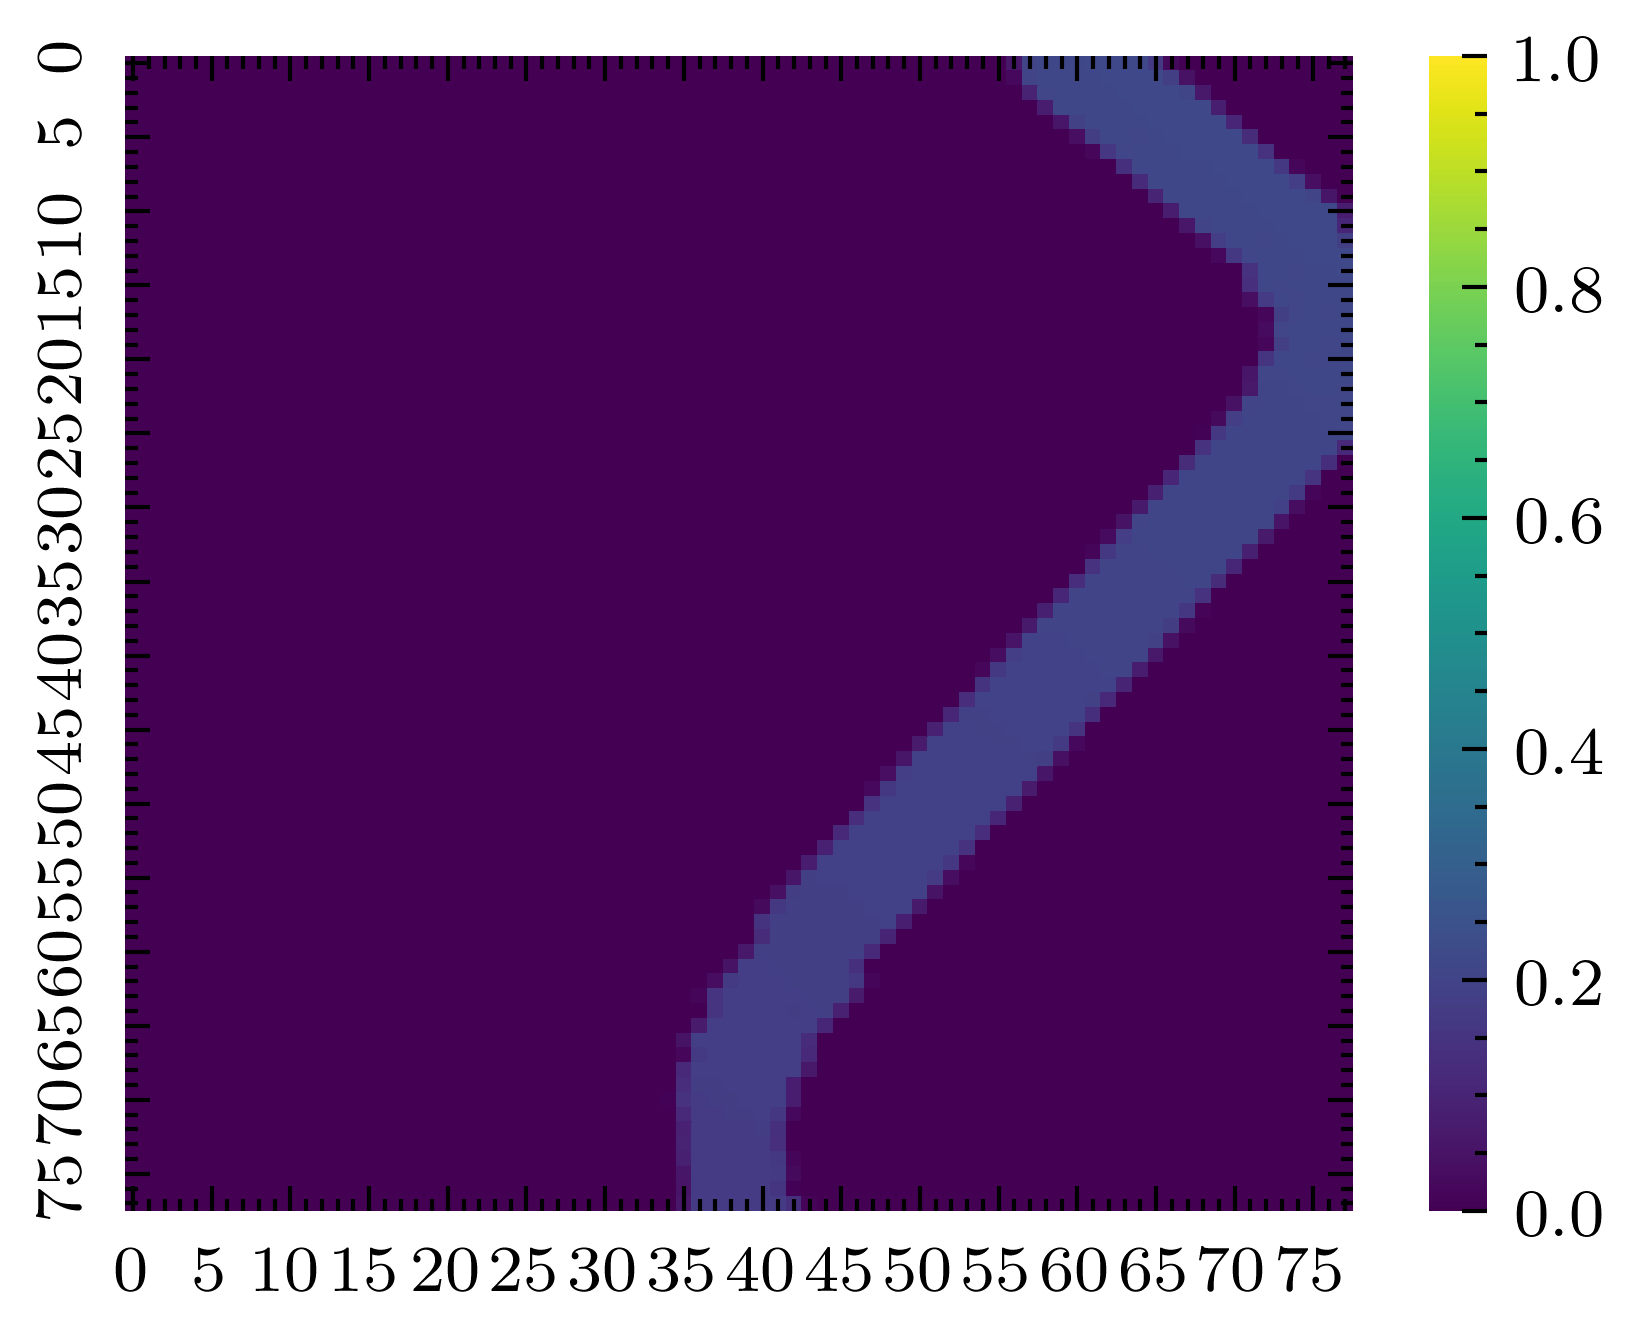
\includegraphics[width=\linewidth]{../img/bars1-example-patches/2d/7.png}    
    \end{subfigure}  
    \begin{subfigure}[b]{0.19\textwidth}
    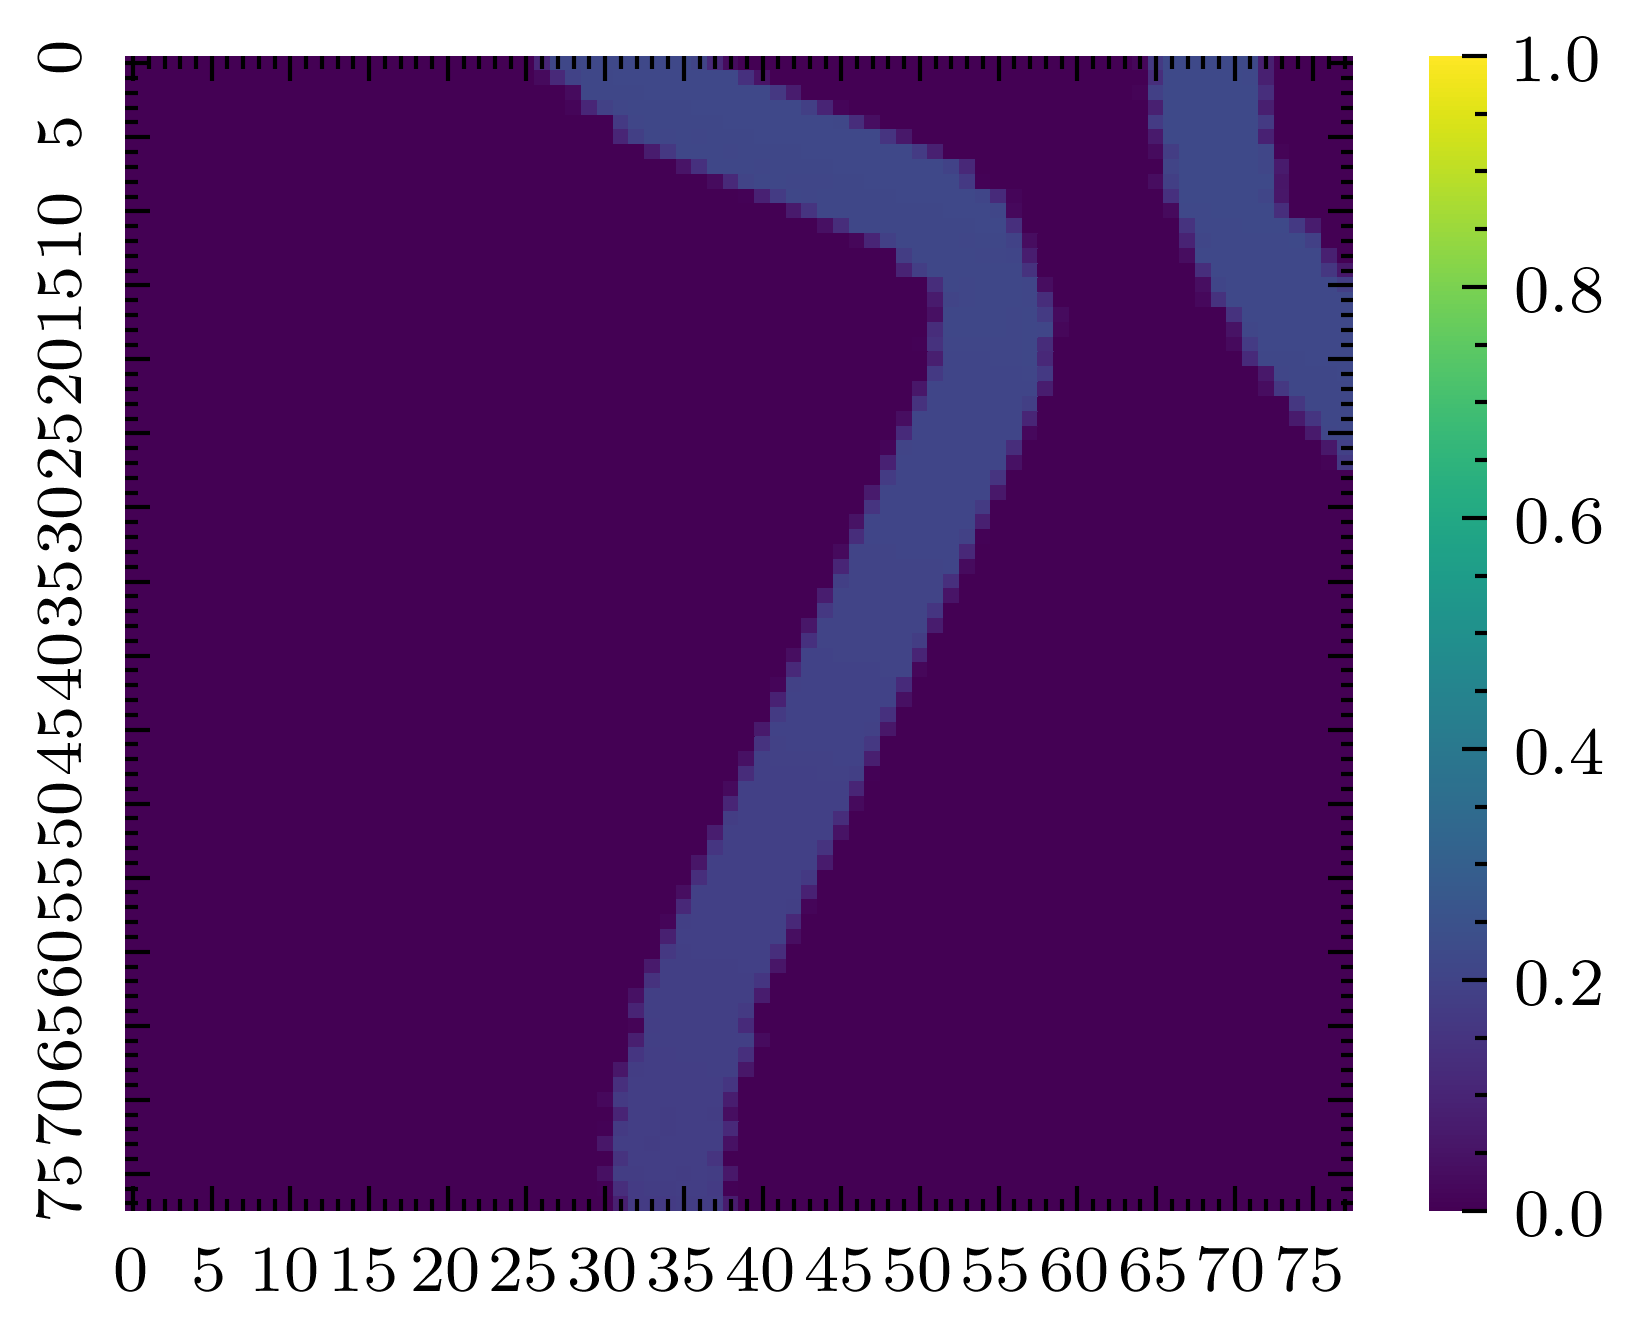
\includegraphics[width=\linewidth]{../img/bars1-example-patches/2d/14.png}    
    \end{subfigure}  
\caption{Cropped patches in 2D.}
\end{subfigure}  
\begin{subfigure}[b]{1\textwidth}
    \begin{subfigure}[b]{0.19\textwidth}
    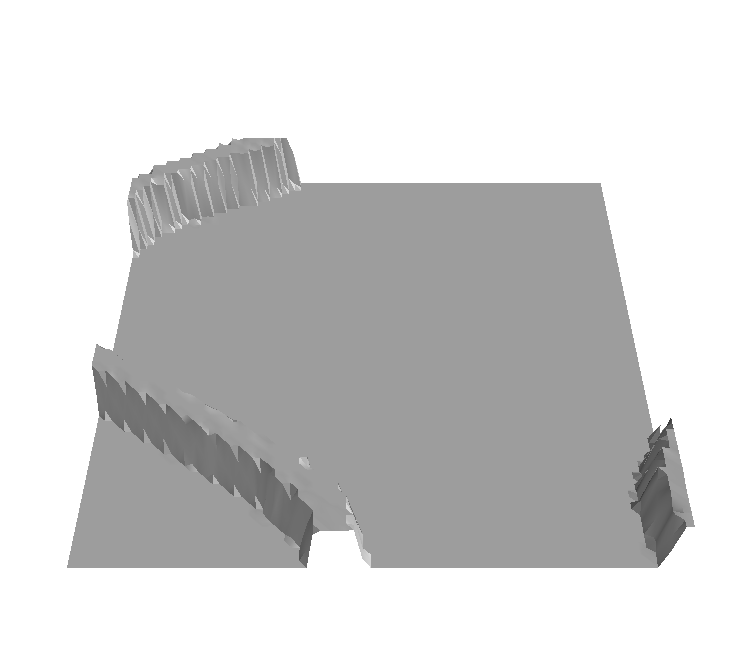
\includegraphics[width=\linewidth]{../img/bars1-example-patches/3d/0.png}
    \end{subfigure}
    \begin{subfigure}[b]{0.19\textwidth}
    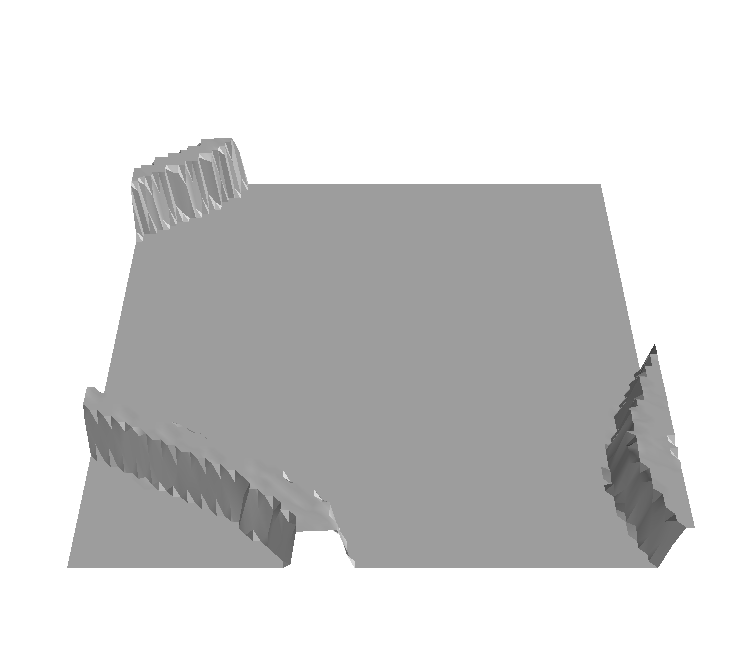
\includegraphics[width=\linewidth]{../img/bars1-example-patches/3d/2.png}    
    \end{subfigure}  
    \begin{subfigure}[b]{0.19\textwidth}
    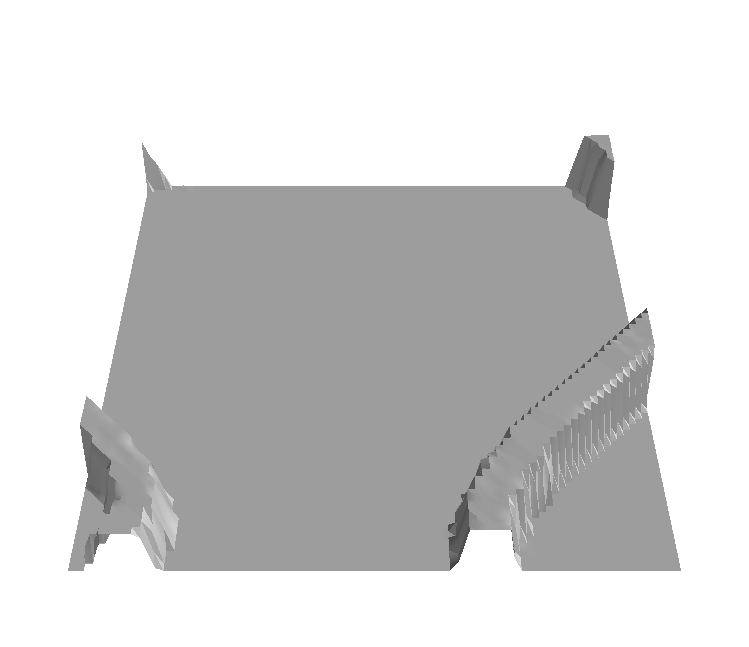
\includegraphics[width=\linewidth]{../img/bars1-example-patches/3d/4.png} 
    \end{subfigure}
    \begin{subfigure}[b]{0.19\textwidth}
    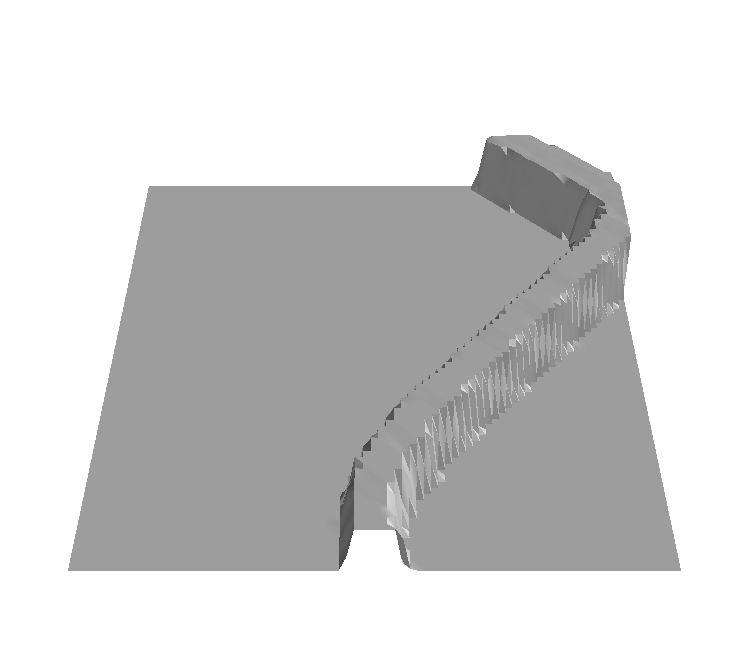
\includegraphics[width=\linewidth]{../img/bars1-example-patches/3d/7.png}    
    \end{subfigure}  
    \begin{subfigure}[b]{0.19\textwidth}
    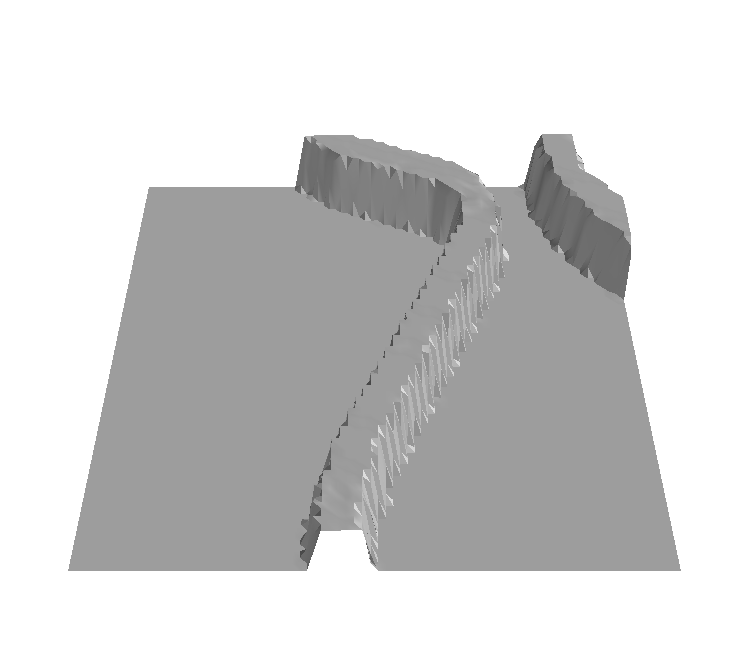
\includegraphics[width=\linewidth]{../img/bars1-example-patches/3d/14.png}    
    \end{subfigure}  
\caption{Cropped patches in 3D.}
\end{subfigure}
\caption{Example of a robot trajectory (a) extracted during training on a map with different walls. Robot's initial position is showed by its white siluette. Patches borders are label with greed if traversable and red if not and showed as 2D (b) and 3D(c) rendered images.}
\end{figure}

We used deep learning techiques to directly lean features from raw data, in our case images, without needing to preprocess the inputs as it was done historically.


\begin{figure}[H]
    \centering
        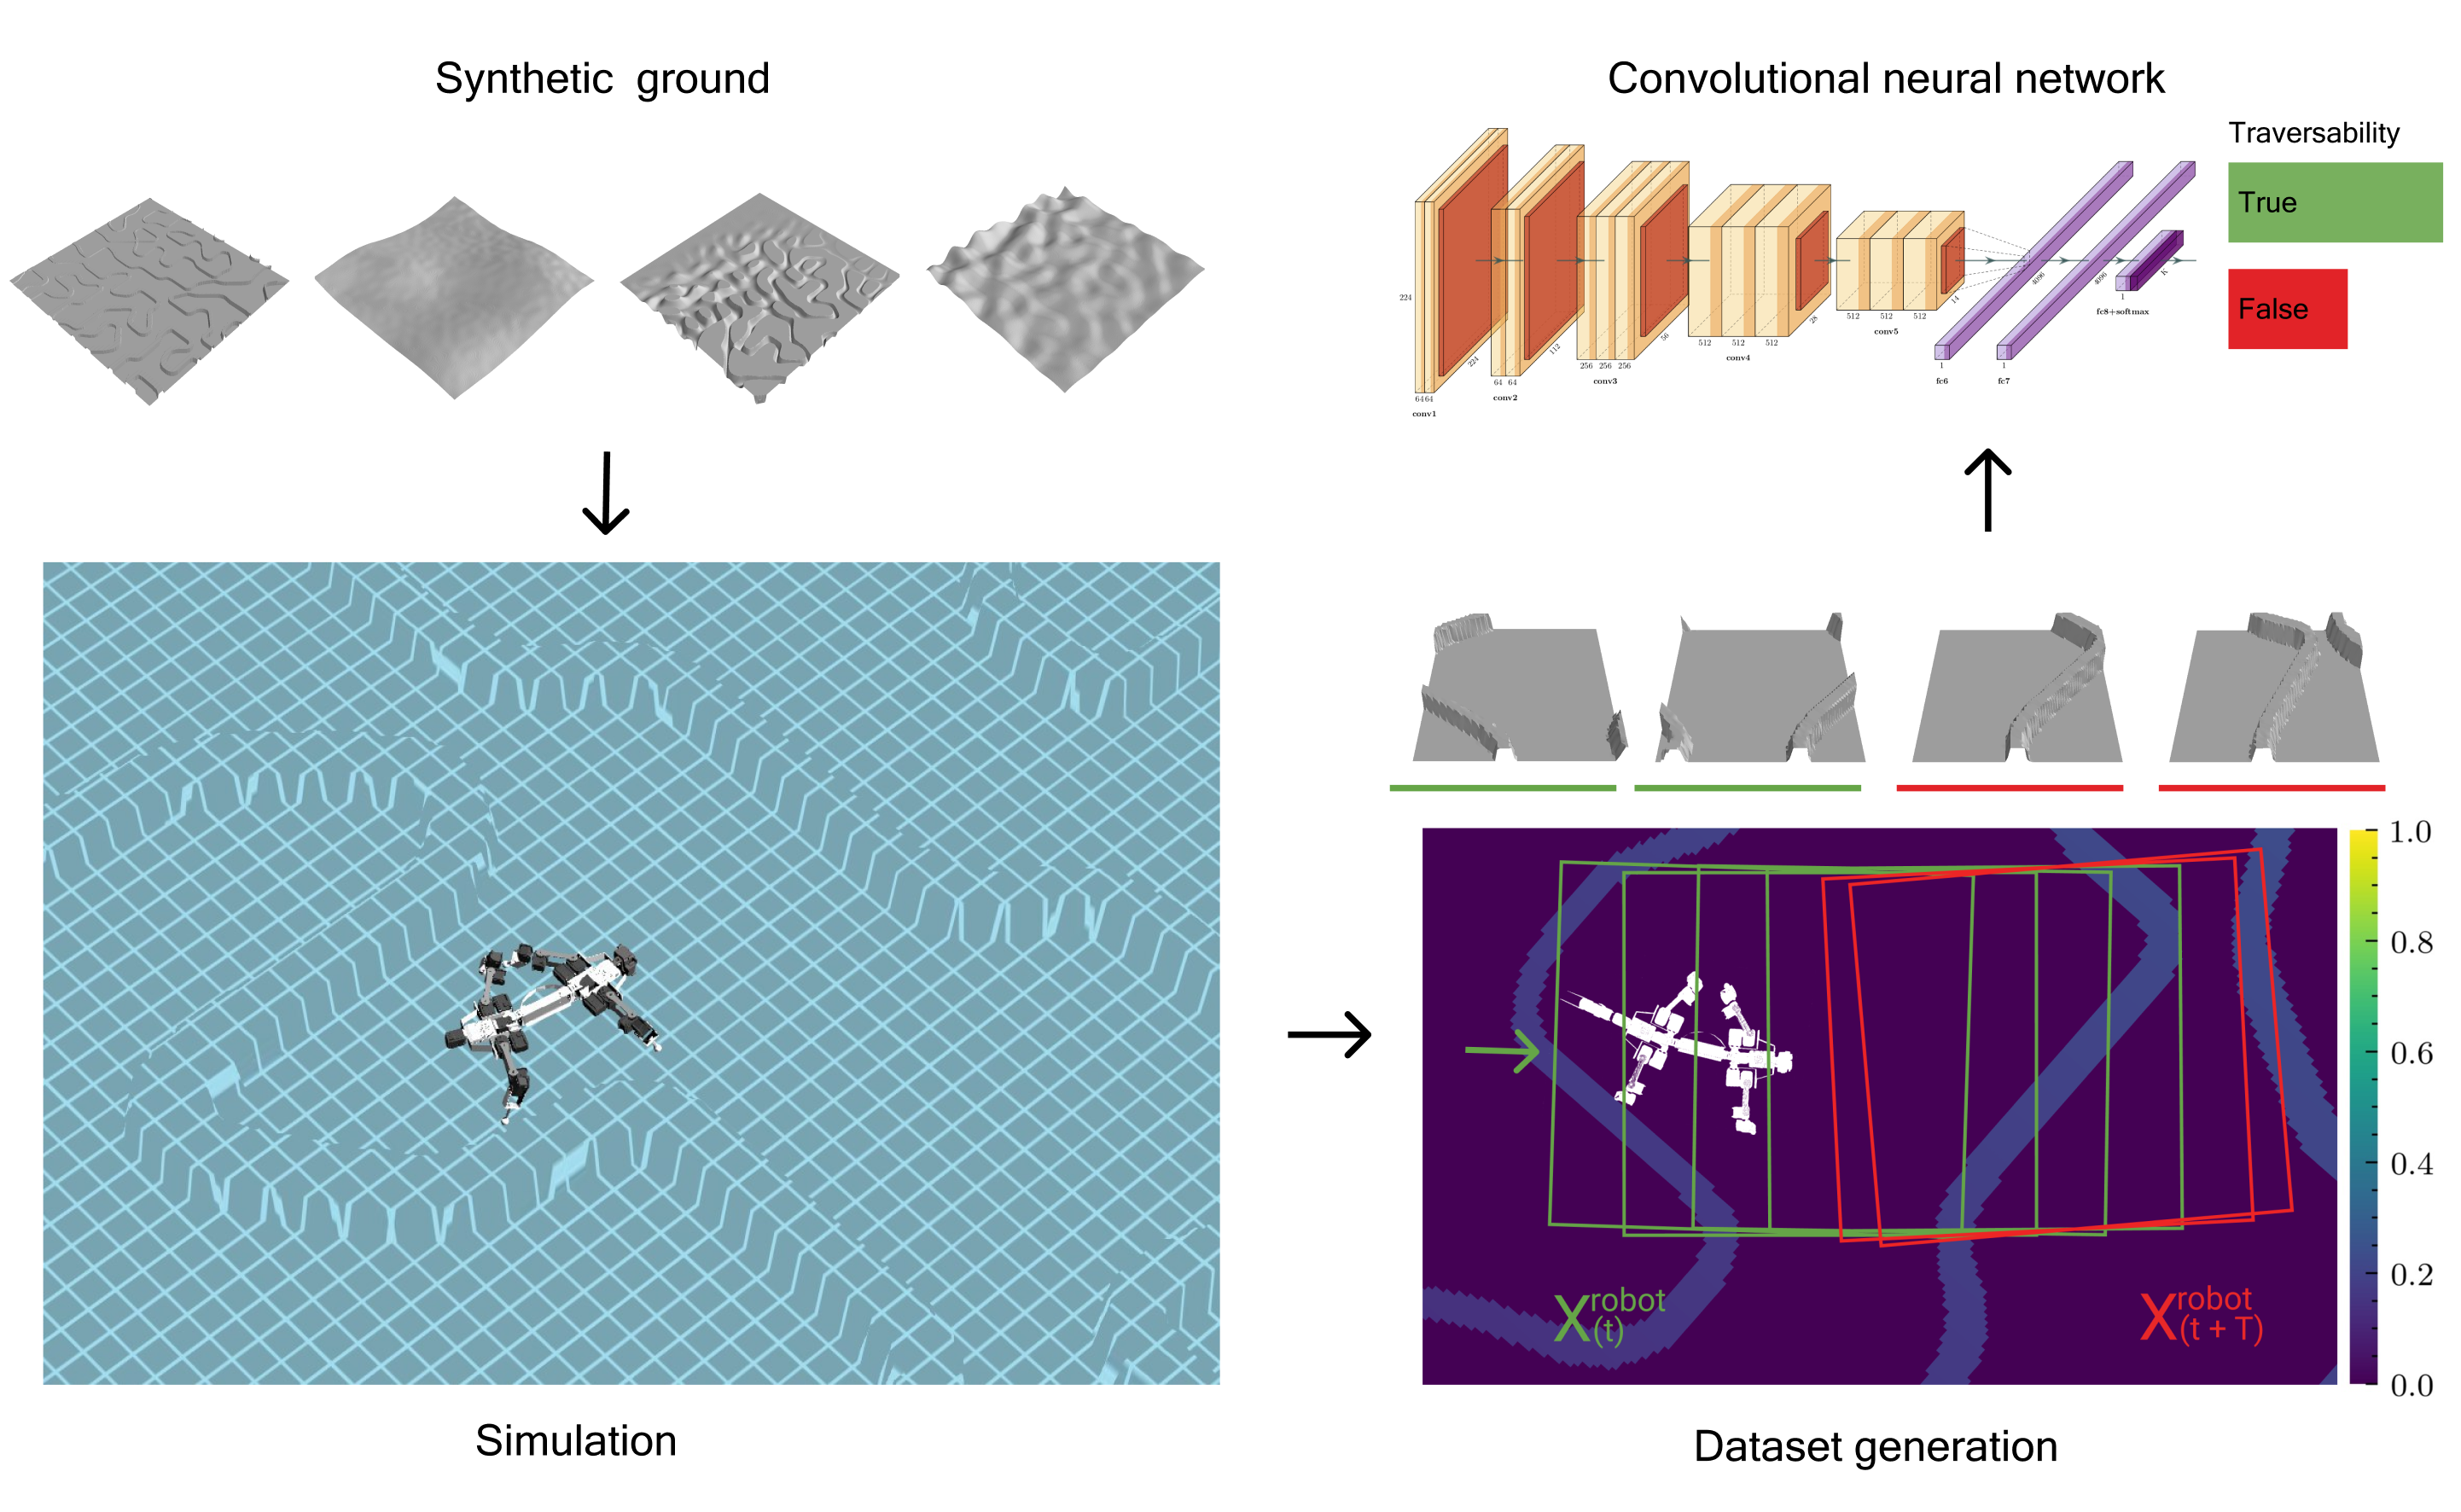
\includegraphics[width=\textwidth]{../img/method.png}
    \caption{The proposed traversability framework's main blocks in couter-clockwise order. First we generated meaningful synthetic ground, then we let the robot spawn and walk on them in simulated enviroment while storing its interactions. Later, we crop a region of ground, a patch, for each simulation trajectory around the robot according to its locomotion. We label those images using a defined treshold and fit a deep convolutional neural network to predict traversability. }
    \end{figure}

    \begin{figure}[H]
    \centering
        
    \begin{subfigure}[b]{0.19\textwidth}
        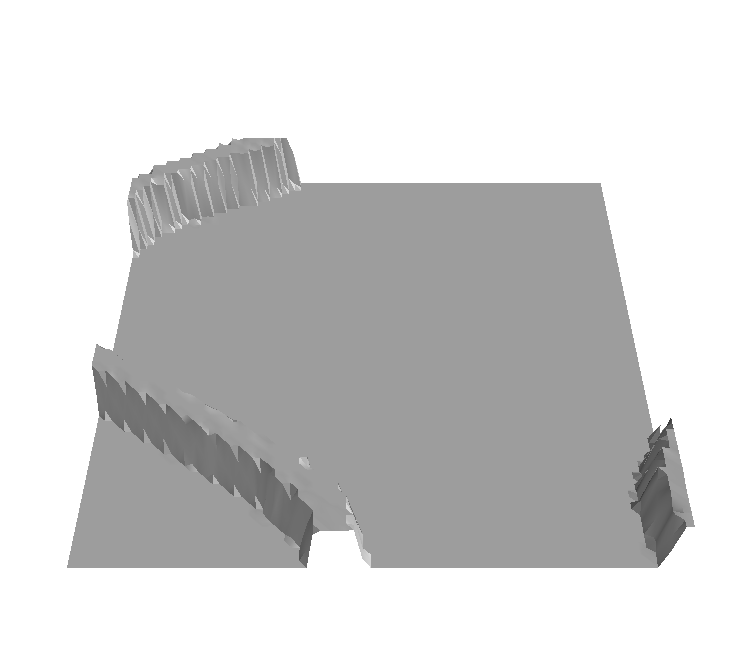
\includegraphics[width=\linewidth]{../img/bars1-example-patches/3d/0.png}
    \end{subfigure}
    \begin{subfigure}[b]{0.19\textwidth}
    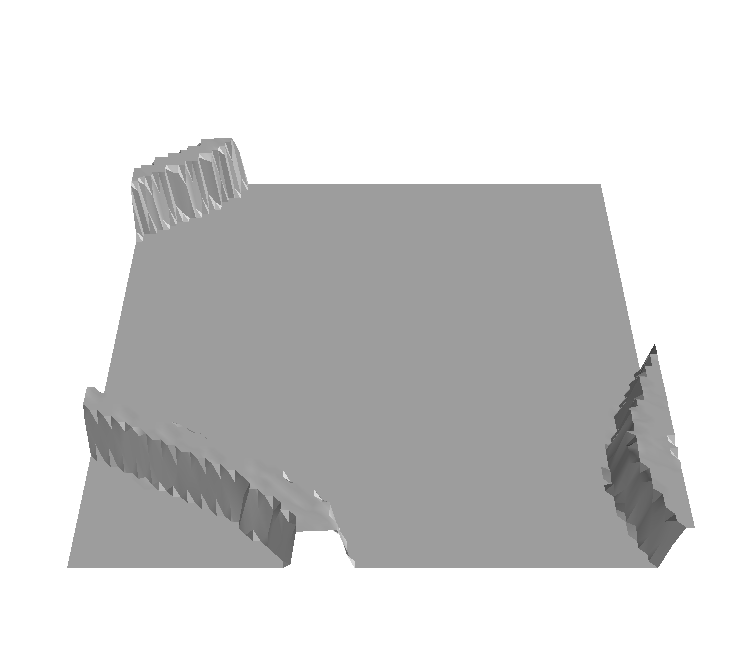
\includegraphics[width=\linewidth]{../img/bars1-example-patches/3d/2.png}    
\end{subfigure}  
    \begin{subfigure}[b]{0.19\textwidth}
    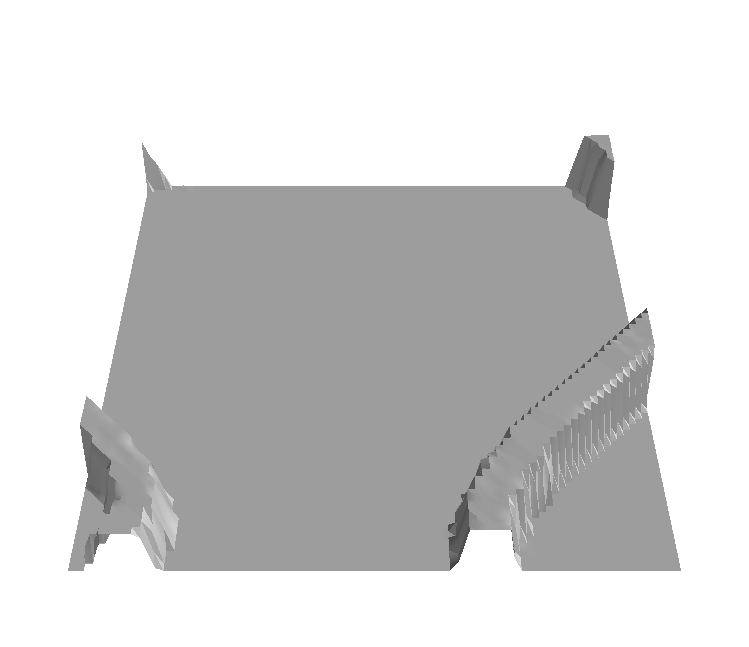
\includegraphics[width=\linewidth]{../img/bars1-example-patches/3d/4.png}    
\end{subfigure}
    \begin{subfigure}[b]{0.19\textwidth}
    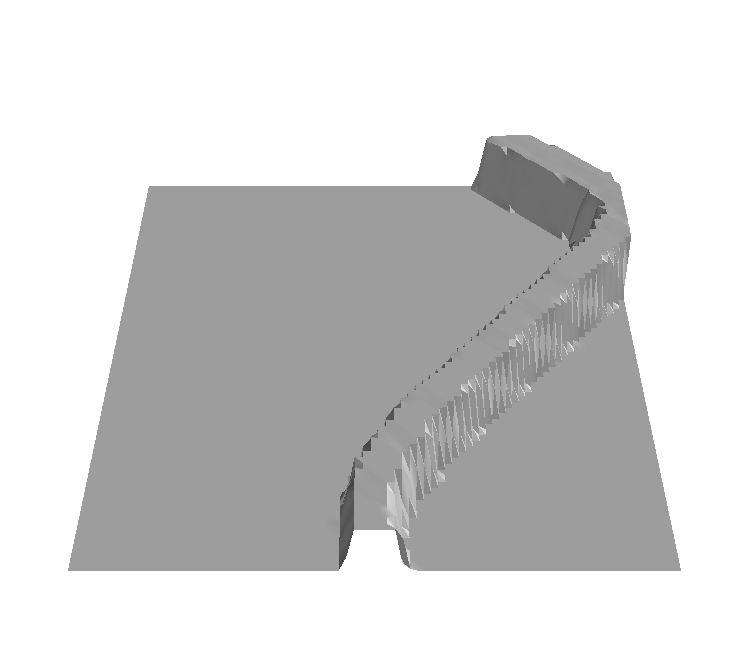
\includegraphics[width=\linewidth]{../img/bars1-example-patches/3d/7.png}    
\end{subfigure}  
    \begin{subfigure}[b]{0.19\textwidth}
    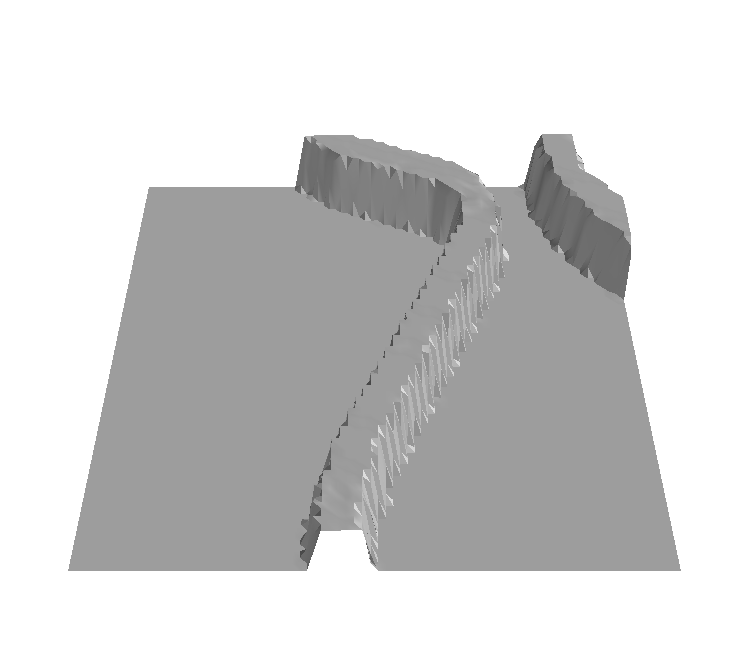
\includegraphics[width=\linewidth]{../img/bars1-example-patches/3d/14.png}    
\end{subfigure}  
    \end{figure}

\begin{figure}[H]
    \centering
    \begin{subfigure}[b]{0.19\textwidth}
        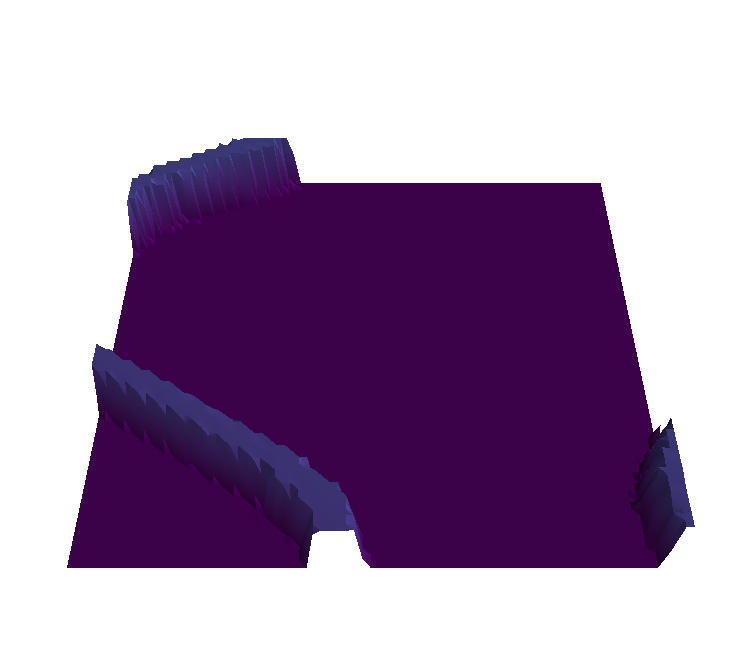
\includegraphics[width=\linewidth]{../img/bars1-example-patches/3d-viridis/0.png}
    \end{subfigure}
    \begin{subfigure}[b]{0.19\textwidth}
    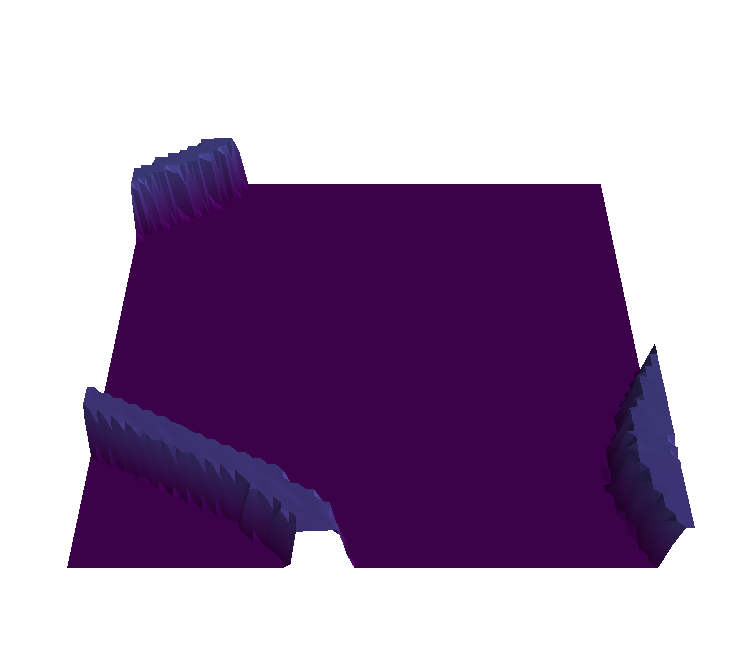
\includegraphics[width=\linewidth]{../img/bars1-example-patches/3d-viridis/2.png}    \end{subfigure}  
    \begin{subfigure}[b]{0.19\textwidth}
    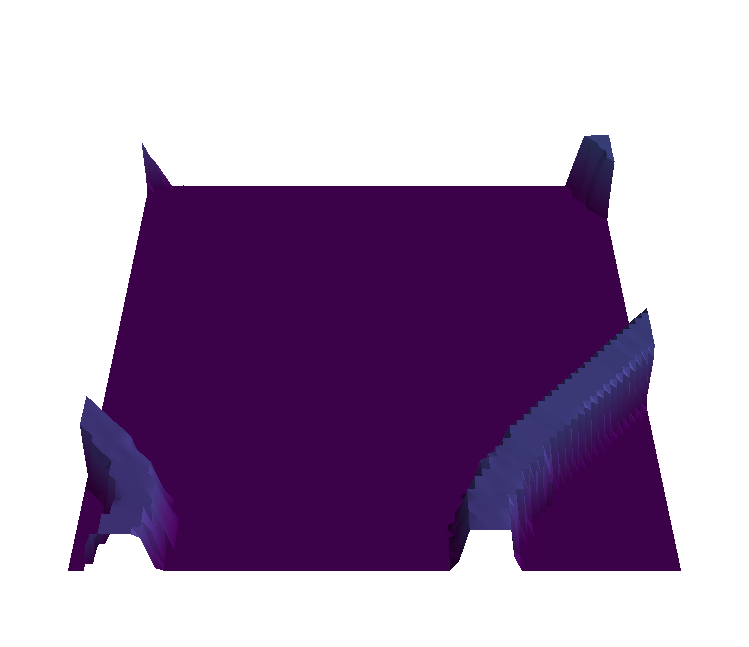
\includegraphics[width=\linewidth]{../img/bars1-example-patches/3d-viridis/4.png}    \end{subfigure}
    \begin{subfigure}[b]{0.19\textwidth}
    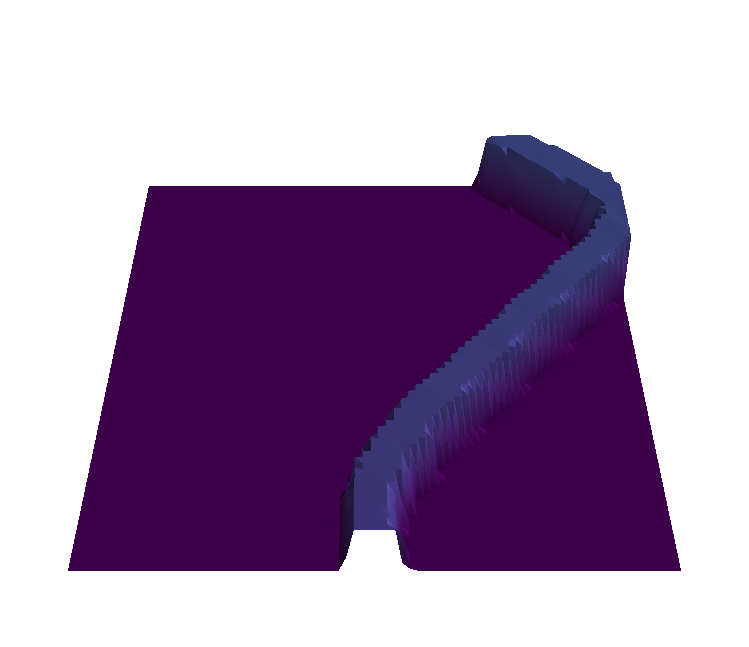
\includegraphics[width=\linewidth]{../img/bars1-example-patches/3d-viridis/7.png}    \end{subfigure}  
    \begin{subfigure}[b]{0.19\textwidth}
    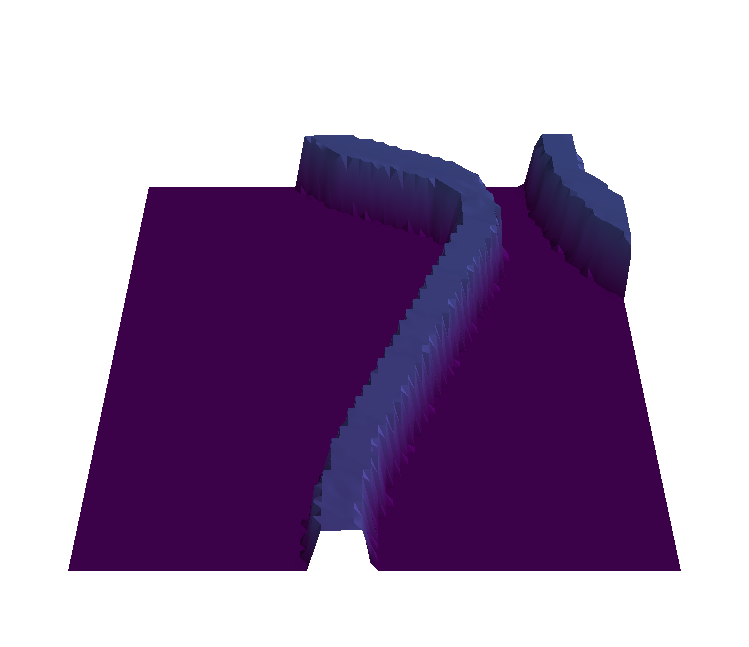
\includegraphics[width=\linewidth]{../img/bars1-example-patches/3d-viridis/14.png}    \end{subfigure}  

\end{figure}

\end{document}
